\documentclass[a4paper,12pt]{article}

\usepackage[colorlinks,unicode]{hyperref}
\usepackage[affil-it]{authblk}
\usepackage[rgb]{xcolor}
\hypersetup{				% Гиперссылки
    colorlinks=true,       	% false: ссылки в рамках
	urlcolor=blue           % на URL
}

%  Русский язык
\usepackage[T2A]{fontenc}			% кодировка
			% кодировка исходного текста
\usepackage[english,russian]{babel}	% локализация и переносы
\usepackage[utf8]{inputenc}

% Footnotes
\usepackage[bottom]{footmisc}

% Математика
\usepackage{amsmath,amsfonts,amssymb,amsthm,mathtools}
\usepackage{thmtools}
\usepackage{cases}

\usepackage{physics}
\usepackage{cleveref}

% Mathematical formating
\newtheorem{theorem}{Теорема}
\theoremstyle{definition}
\newtheorem{definition}{Определение}[section]
\renewcommand{\theoremautorefname}{теоремы}

% Add lemma support
\newtheorem{lemma}{Лемма}
\newtheorem{sublemma}{Лемма}[lemma]

\usepackage{wasysym}

%Заголовок
\author{Мирзоев С.Е.%
\thanks{E-mail: \texttt{mrsergeymirzoev@gmail.com}}}
\title{Оценка бессрочных опционов для случайных процессов со скачками}
\affil{Факультет Вычислительной Математики и Кибернетики, Московский государственный университет им. М.В.Ломоносова}

\makeatletter
% Roman numbers support
\newcommand*{\rom}[1]{\expandafter\@slowromancap\romannumeral #1@}

% Derivative at point support
\newcommand{\at}[2][]{#1|_{#2}}

% Expectation support
\newcommand{\expect}{\operatorname{E}\expectarg}
\DeclarePairedDelimiterX{\expectarg}[1]{[}{]}{%
  \ifnum\currentgrouptype=16 \else\begingroup\fi
  \activatebar#1
  \ifnum\currentgrouptype=16 \else\endgroup\fi
}

\newcommand{\innermid}{\nonscript\;\delimsize\vert\nonscript\;}
\newcommand{\activatebar}{%
  \begingroup\lccode`\~=`\|
  \lowercase{\endgroup\let~}\innermid 
  \mathcode`|=\string"8000
}

\renewcommand\qedsymbol{$\blacksquare$}

\makeatother

\begin{document}

\begin{titlepage}
\centering

\textsc{Дипломная работа}

\vspace{\stretch{1}}

{\LARGE\bfseries Оценка бессрочных колл-опционов для случайных процессов со скачками\\}
\rule{3in}{0.4pt}

\vspace{\stretch{1}}

\textbf{Мирзоев С.Е.}\\
Московский государственный университет им. М.В.Ломоносова\\
Факультет Вычислительной Математики и Кибернетики\\
Март 2022

\vspace{\stretch{1}}

{\small
Научный руководитель: Белянкин Г.А.\\
Со-руководитель: Морозов В.В.}

\vspace*{\stretch{1}}

\end{titlepage}
\thispagestyle{empty}

\newpage
\tableofcontents

\newpage

%%%%%%%%%%%%%%%%%%%%%%%%%%%%%%%%%%%%
%%%%%%%%%%%%% Введение %%%%%%%%%%%%%
%%%%%%%%%%%%%%%%%%%%%%%%%%%%%%%%%%%%
\section{Введение}

В статье Гербера и Шиу была сделана оценка бесконечного пут-опциона, в данной статье аналогичный результат будет получен для колл-опциона. Как и в указанной статье, в данной работе рассматриваются две модели, в которых логарифм цены актива представляет собой смещённый сложный пуассоновский процесс. Явные результаты получены для цен и оптимальных стратегий исполнения определенных бессрочных американских опционов на актив, в частности для бессрочного колл-опциона. В первой модели, в которой скачки цены актива направлены вверх, результаты получаются с использованием процесса - мартингала и условия гладкого сшивания. Во второй модели, в которой скачки идут вниз, показывается, что значение стратегии, соответствующее постоянной границе исполнения опциона удовлетворяет определенному уравнению обновления. Будет получена оптимальная стратегию исполнения, удовлетворяющая условию непрерывного сшивания. Кроме того, одна и та же модель может быть использована для определения цены на определенные параметры отмены. Наконец, было показано, как классическая модель геометрического броуновского движения может быть использована в качестве предела, а также, как она может быть встроена в обе модели.

%%%%%%%%%%%%%%%%%%%%%%%%%%%%%%%%%%%%
%%%%%%%% Постановка задачи %%%%%%%%%
%%%%%%%%%%%%%%%%%%%%%%%%%%%%%%%%%%%%

\section{Постановка задачи}

Пусть $S(t)$ - цена актива, например, акции, в момент времени $t \ge 0$. Мы предполагаем, что рынок риск-нейтрален, следовательно, стоимость ценной бумаги - это математическое ожидание дисконтированных будущих платежей. В предположении, что по активу не выплачивается никаких дивидендов и что безрисковая мгновенная процентная ставка $r$ является положительной константой, случайный процесс $\{e^{-rt} S(t)\}$, представляющий собой дисконтированную цену актива  является мартингалом.

Пусть $U(t) = \ln{S(t)}, t \ge 0$. Мы предполагаем, что $\{U(t), t \ge 0\}$ - процесс с независимыми и стационарными приращениями, с начальным значением $U(0) = \ln{S(0)} = \ln{s} = u$. Классическая модель цены акции является частным случаем, в котором $\{U(t)\}$ представляет собой винеровский процесс со сдвигом $\mu = r - \frac{\sigma ^ {2}}{2}$ и бесконечно малой дисперсией $\sigma ^ {2}$. 

\newpage

В данной работе будут рассмотрены две модели:

\textbf{Модель \rom{1}:}
\begin{equation}\label{eq:model1_definition}
    U(t) = u - ct + Z(t)
\end{equation}

\textbf{Модель \rom{2}\footnote{Заметим, что модель \rom{2} напоминает модель, которая используется для процесса избытка в классической теории риска.}:} 
\begin{equation}\label{eq:model2_definition}
    U(t) = u + ct - Z(t)
\end{equation}

В обоих случаях $c > 0$ и является постоянной величиной, а $\{Z(t)\}$ представляет собой сложный пуассоновский процесс, определяемый параметром $\lambda > 0$ и распределением величин скачка. Заметим также, что скачки положительны.

\label{sec:positivityOfJumsAssumption} Для упрощения обозначений предположим, что распределения величин скачка
непрерывны с плотностью вероятности $p(x), x \ge 0$. 

\subsection{Сложный пуассоновский процесс}

Перед тем, как далее исследовать предложенные модели, стоит уточнить, что такое сложный пуассоновский процесс, а также получить важные результаты, связанные с ним.

\begin{definition}[Сложный пуассоновский процесс]
    \label{def:compound_poisson}
    Процесс $\{X_t, t \ge 0\}$ называется \textbf{сложным процессом Пуассона}, если мы можем записать его как:
    
    \begin{equation}
        X_t = \sum_{i=1}^{N_t} Y_i,
    \end{equation}
    
    где $\{N_t, t \ge 0\}$ - процесс Пуассона, а $\{Y_n\}_{n \ge 1}$ - семейство случайных независимых v. с тем же распределением, которые также независимы от $\{N_t, t \ge 0\}$.
\end{definition}

\begin{definition}\label{def:moment_generating_function}
Через \textbf{производящую функцию моментов} случайной величины $X$ будем обозначать:
    \begin{equation*}
        M_X(\alpha) = \expect{e^{\alpha X}}
    \end{equation*}
\end{definition}

\begin{lemma}\label{thm:thm2_moment_generating_function}
Производящая функция сложного Пуассоновского процесса $\{X(t)\}$ равна:

\begin{equation}\label{eq:moment_generating_for_poisson}
     M_{X(t)}(\alpha) = e^{\lambda t \left(M_{Y_1}(\alpha) - 1\right)}
\end{equation}

\end{lemma}

\begin{proof}

Распишем производящую функцию моментов для обобщенного Пуассоновского процесса:

\begin{equation*}
     M_{X_t}(\alpha) = \expect[\big]{e^{\alpha X_t}} = \expect[\big]{e^{\alpha \sum_{i=1}^{N_t} Y_i}}
\end{equation*}

Также заметим, что распределение $N_t$ нам известно:

\begin{equation}\label{eq:thm2_moment_generating_function_eq1}
     \expect[\big]{e^{\alpha \sum_{i=1}^{N_t} Y_i}} = \sum_{m=0}^{\infty} \expect[\big]{e^{\alpha \sum_{i=1}^{m} Y_i}} P(N_t = m) = \sum_{m=0}^{\infty} \expect[\big]{e^{\left(\alpha \sum_{i=1}^{m} Y_i\right)}} \frac{(\lambda t)^{m} e^{-\lambda t}}{m!}
\end{equation}

Так как случайные величины $Y_i$ независимы и одинаково распределены, верно:

\begin{equation}\label{eq:thm2_moment_generating_function_eq2}
     \expect[\big]{e^{\alpha \sum_{i=1}^{m} Y_i}} = \expect[\big]{\prod_{i=1}^{m} e^{\alpha Y_i}} = \prod_{i=1}^{m}  \expect[\big]{e^{\alpha Y_i}} = \prod_{i=1}^{m}  \expect[\big]{e^{\alpha Y_1}} = \left( \expect[\big]{e^{\alpha Y_1}} \right)^{m}
\end{equation}

Далее необходимое получается при подстановке \eqref{eq:thm2_moment_generating_function_eq1} и \eqref{eq:thm2_moment_generating_function_eq2} в цепочку уравнений:

\begin{equation*}
\begin{split}
    \sum_{m=0}^{\infty} \expect{e^{\left(\alpha \sum_{i=1}^{m} Y_i\right)}} \frac{(\lambda t)^{m} e^{-\lambda t}}{m!} &= \sum_{m=0}^{\infty} \left(\expect{e^{\alpha Y_1}}\right)^{m} \frac{(\lambda t)^{m} e^{-\lambda t}}{m!} =\\
    = \sum_{m=0}^{\infty} (M_{Y_1} (\alpha))^{m} \frac{(\lambda t)^{m} e^{-\lambda t}}{m!} &= \sum_{m=0}^{\infty} \frac{(M_{Y_1} (\alpha) \lambda t)^{m}}{m!} e^{-\lambda t} =\\
    = e^{\left(M_{Y_1} (\alpha) \lambda t\right)} e^{-\lambda t} &= e^{\lambda t \left(M_{Y_1}(\alpha) - 1\right)}
\end{split}
\end{equation*}

\end{proof}

\subsection{Отсутствие арбитража}

\begin{lemma}[Отсутствие арбитража]\label{thm:no_arbitrage_theoreme}
В модели \rom{2} мы делаем дополнительное предположение, что $c > r$ иначе возникает возможность арбитража. 
\end{lemma}
\begin{proof}
Если бы было допустимо $c \le r$, мы бы имели $S(t) \le s e^{rt}$ со строгим неравенством после первого скачка, т.к. скачки положительны. Следовательно, путем короткой продажи (Подробнее: \ref{def:short_position}) актива и инвестирования выручки $s$ по безрисковой процентной ставке $r$ мы могли бы получить безрисковую прибыль.

Действительно, пусть в момент $\tau = 0$ инвестор берёт актив в короткую позицию, сразу её продаёт и сумму $S(\tau)$ кладёт на депозит в банк под ставку $r$. Далее он ждёт, когда произойдет первый скачок актива и выполнится $e^{rt} S(\tau) > S(t)$. После выполнения этого условия, инвестор забирает деньги с банковского депозита, покупает актив, возвращает его брокеру и имеет безрисковую прибыль $e^{rt}S(\tau) - S(t) = s e^{rt} - S(t)$.
\end{proof}

Наша главная цель - оценить бессрочный американский
опцион с функцией выплаты $P(s)$. Хотя указание \textit{американский} не является обязательным, оно добавляется, чтобы подчеркнуть, что опцион может быть исполнен в любой момент.

\subsection{Оптимальная стратегия исполнения}

Если такой опцион будет исполнен в момент времени $T$, прибыль составит $P(S(T))$. Ограничимся колл-опционами с функциями выплаты, для которых априори ясно, что оптимальными стратегиями исполнения будут моменты остановки вида:

\begin{equation}\label{eq:optimal_excersize}
T_L = \inf\limits_{S(t) > L}{t}
\end{equation}

Здесь граница исполнения опциона $L$ является положительной константой. Также заметим, что $L > K$, иначе исполнение опциона никогда не будет производиться - мы будем покупать по рыночной цене $L$. 

%%%%%%%%% Model I logarithmic track graph

\begin{figure}[htbp]
\label{fig:model1track}
\centerline{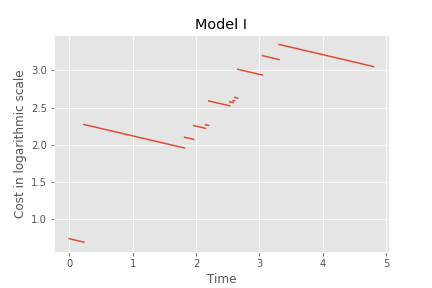
\includegraphics[scale=0.7]{img/model1.png}}
\caption{График U(t) для модели \rom{1}}
\end{figure}

Оптимальность данной стратегии исполнения, в частности, справедлива для бессрочного \textbf{колл-опциона} со \textbf{"страйком"} (ценой исполнения) $K$:

\begin{equation}\label{eq:payoff_function}
P(s) = \max(s - K, 0) = (s - K)_+,
\end{equation}

Проблема состоит в том, чтобы сначала найти стоимость стратегии $T_L$. Будем рассчитывать её, как математическое ожидание приведённого к настоящему моменту платежа по опциону, то есть:

\begin{equation}\label{eq:strategy_cost}
V(s; L) = \expect*{e^{-rT_L} P(S(T_L)) | S(0) = s}, s \le L,
\end{equation}

Затем определим оптимальное значение $\widetilde{L}$, которое максимизирует $V(s; L)$. Такое значение $\widetilde{L}$ - оптимальная граница опциона. Итак, стоимость опциона равна:

\begin{equation}\label{eq:option_price}
    \begin{cases}
      V(s; \widetilde{L}), \text{ при } s \le \widetilde{L}\\
      P(s), \text{ при } s > \widetilde{L}
    \end{cases}\,.
\end{equation}

%%%%%%%%%%%%%%%%%%%%%%%%%%%%%%%%%%%%
%%%%%% Решение для модели 1 %%%%%%%%
%%%%%%%%%%%%%%%%%%%%%%%%%%%%%%%%%%%%
\section{Решение для модели \rom{1}}

%%%%%%%%% Model I logarithmic track graph with cross with log(L)

\begin{figure}[htbp]
\label{fig:model1tracklcrosslog}
\centerline{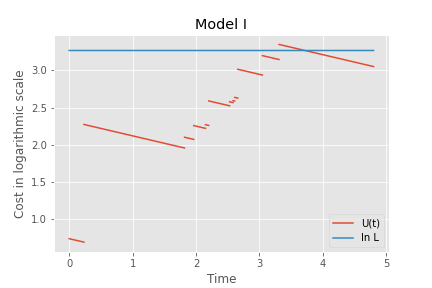
\includegraphics[scale=0.7]{img/model1_with_L_log.png}}
\caption{График пересечения U(t) и ln(L) для модели \rom{1}}
\end{figure}

%%%%%%%%% Model I track graph with cross with L

\begin{figure}[htbp]
\label{fig:model1tracklcross}
\centerline{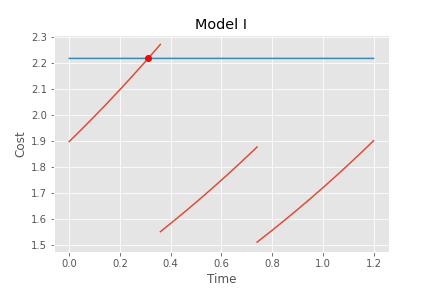
\includegraphics[scale=0.7]{img/model1_with_L.png}}
\caption{График пересечения S(t) и L для модели \rom{1}}
\end{figure}

Поскольку \hyperref[fig:model1tracklcross]{траектория} процесса $\{S(t)\}$ не имеют скачков вниз, точная нижняя грань \eqref{eq:optimal_excersize} достигается на непрерывном участке траектории. Это означает, что $S(T_L) = L$, и, следовательно, \eqref{eq:strategy_cost} получает вид:

\begin{equation}\label{eq:strategy_c1}
V(s; L) = P(L) \expect*{e^{-rT_L} | S(0) = s}, s \le L,
\end{equation}

В \eqref{eq:strategy_c1} остается определить мат.ожидание. Для этого решим вспомогательную задачу - найдём все такие $\xi$, при которых случайный процесс $\{e^{-rt}S(t)^{\xi}\}$ является мартингалом.

\begin{theorem}[Мартингальное условие для $\xi$]\label{thm:martingale_cond_for_xi}
Пусть для некоторого $\xi$, случайный процесс $\{e^{-rt}S(t)^{\xi}\}$ является мартингалом. Тогда мартингальное условие имеет вид:

\begin{equation}\label{eq:martingale_cond_for_xi_log}
\lambda \left[ \int_{0}^{+\infty} e^{\xi x} p(x) \,dx - 1  \right] - r - c \xi
 = 0
\end{equation}

\end{theorem}

\begin{proof}
Классическое мартингальное условие для $\{e^{-rt} S(t)^{\xi}\}$:

\begin{equation*}
\expect*{e^{-rt} S(t)^{\xi}|S(0) = s} = s^{\xi}
\end{equation*}

Учитывая определение процесса $\{U(t)\}$:

\begin{equation*}
\expect*{e^{-rt + \xi U(t)}|U(0) = u} = e^{\xi u}
\end{equation*}

Так как $\{U(t), t \ge 0\}$ - процесс с независимыми и стационарными приращениями, условие мартингальности для указанного процесса с произвольным $\xi$ при $t = 1$\footnote{выбор конкретного момента реализации процесса $t=1$ не сужает общности решаемой задачи} выглядит как:
\begin{equation*}\label{eq:thm2_eq1}
e^{-r}\expect*{e^{\xi U(1)}} = e^{\xi u}
\end{equation*}

Из формулировки первой модели \eqref{eq:model1_definition}, уравнение выше принимает вид:

\begin{equation*}
e^{-r}\expect*{e^{\xi(u - c + Z(1))}} = e^{\xi u}
\end{equation*}

Откуда можно вынести неслучайные составляющие:

\begin{equation*}
e^{-r - c \xi} \expect*{e^{\xi Z(1)}} = 1
\end{equation*}

Заметим, что математическое ожидание в выражении выше представляет собой производящую функцию моментов обобщенного пуассоновского процесса\textsuperscript{{\ref{def:compound_poisson}}}:

\begin{equation*}
e^{-r - c \xi} M_{Z(1)}(\xi) = 1
\end{equation*}

Теперь прологарифмируем обе части:

\begin{equation*}
\ln{M_{Z(1)}(\xi)} - r - c\xi = 0
\end{equation*}

И применим результат леммы \ref{thm:thm2_moment_generating_function}:

\begin{equation*}
\ln{e^{\lambda (M_{Y_1}(\xi) - 1)}} - r - c\xi = 0
\end{equation*}

Раскрыв логарифм, получим:

\begin{equation}\label{eq:thm2_eq2}
\lambda \left(M_{Y_1}(\xi) - 1\right) - r - c\xi = 0
\end{equation}

Заметим, что $M_{Y_1}(\xi)$, производящая функция моментов\textsuperscript{{\ref{def:moment_generating_function}}}, нам известна:

\begin{equation*}
M_{Y_1}(\xi) = \expect{e^{\xi Y_1}} = \int_{0}^{+\infty} e^{\xi x} p(x) \,dx
\end{equation*}

Подставим производящую функцию моментов скачка в \eqref{eq:thm2_eq2} и получим требуемое:
\begin{equation*}
\lambda \left(\int_{0}^{+\infty} e^{\xi x} p(x) \,dx - 1\right) - r - c\xi = 0
\end{equation*}
\end{proof}

Далее сформулируем утверждение о виде функции в левой части уравнения \eqref{eq:martingale_cond_for_xi_log}.

%%%%%%%%% Model I martingale condition

\begin{figure}[htbp]
\label{fig:model1martingalecond}
\centerline{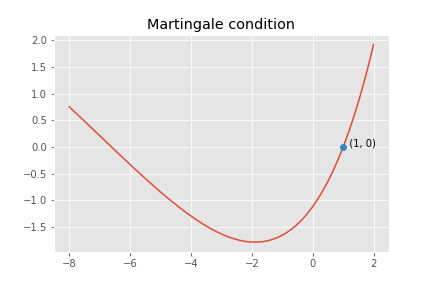
\includegraphics[scale=0.7]{img/model1_martingale_cond.png}}
\caption{Пример графика функции мартингального условия для модели \rom{1}}
\end{figure}

\begin{lemma}[Строгая выпуклость]\label{thm:strict_convexity_m1}
Выражение в левой части уравнения \eqref{eq:martingale_cond_for_xi_log} является строго выпуклой функцией по $\xi$.
\end{lemma}
\begin{proof}
Рассмотрим вторую производную данной функции:
\begin{equation*}
\begin{split}
     \pdv[2]{}{\xi} \left[\lambda \left(\int_{0}^{+\infty} e^{\xi x} p(x) \,dx - 1\right) - r - c\xi \right] &= \pdv{}{\xi} \left[\lambda \left(\int_{0}^{+\infty} e^{\xi x} p(x) x \,dx \right) - c \right] =\\
     = \lambda \left(\int_{0}^{+\infty} e^{\xi x} p(x) x^{2} \,dx \right) &= \lambda \expect*{e^{\xi x} x^2}
\end{split}
\end{equation*}

Так как $\lambda > 0$, $x^2 \ge 0$, $e^{\xi x} > 0$, $p(x > 0) \neq 0$, выражение $\lambda \expect*{e^{\xi x} x^2}$ строго положительно, как произведение положительной величины и математического ожидания ненулевой неотрицательной случайной величины. Итак, вторая производная исходной функции строго положительна.

\end{proof}

Учитывая положительность второй производной функции в уравнении \eqref{eq:martingale_cond_for_xi_log}, оно имеет не более двух решений. На самом деле, оно имеет ровно два решения.
\begin{lemma}[О числе решений уравнения \eqref{eq:martingale_cond_for_xi_log}]\label{thm:solution_for_mart_cond_m1}
Уравнение \eqref{eq:martingale_cond_for_xi_log} имеет ровно два решения. \\
Первое: $\xi_1 = 1$, \\
Второе: $\xi_2 = -R < 0$, для некоторого $R > 0$
\end{lemma}
\begin{proof}
Обозначим функцию в левой части уравнения \eqref{eq:martingale_cond_for_xi_log} через $f(\xi)$:
\begin{equation*}
f(\xi) = \lambda \left(\int_{0}^{+\infty} e^{\xi x} p(x) \,dx - 1\right) - r - c\xi
\end{equation*}

Так как ${e^{-rt} S(T), t \ge 0}$ является мартингалом и в то же время является частным случаем процесса  $\{e^{-rt}S(t)^{\xi}\}$ при $\xi_1 = 1$, естественным образом получаем первое решение.

Существование второго решения следует из того, что:

\begin{equation*}
f(0) = \lambda \left(\int_{0}^{+\infty} e^{0} p(x) \,dx - 1\right) - r = \lambda (1 - 1) - r = -r
\end{equation*}

\begin{equation*}
\begin{split}
\lim_{\xi\to-\infty} f(\xi) &= \lim_{\xi\to-\infty} \left[ \lambda \left(\int_{0}^{+\infty} e^{\xi x} p(x) \,dx - 1\right) - r - c\xi \right] =\\
= - \lambda - r - c \xi &= +\infty
\end{split}
\end{equation*}

А так как выражение в левой части - непрерывная функция от $\xi$, она принимает все значения лежащие в $[min(f(\xi)), +\infty)$ на $\xi \in (-\infty, 0]$ по теореме Больцано-Коши о промежуточном значении. Т.к. $min(f(\xi)) < 0$ (минимум достигается, причём не в $\xi = 1$, то есть $min(f(\xi)) < 0$), значит второе пересечение происходит в отрицательной полуоси: $\xi_2 = -R < 0$, для некоторого $R > 0$
\end{proof}

Отметим, что положительный мартингал $\{e^{-rt} S(t)^{-R}\}$ ограничен снизу константой $e^{-r T_L} L^{-R}$ при $t < T_L$. 

Данный факт следует из определения $T_L$ \eqref{eq:optimal_excersize}:
\begin{equation*}
S(t) \le L, \forall t < T_L
\end{equation*}
Значит:
\begin{equation*}
e^{-r T_L} L^{-R} \le e^{-rt}L^{-R} \le e^{-rt}S(t)^{-R}
\end{equation*}

Следовательно, мы можем применить теорему о преобразовании свободного выбора \cite{bib:Shiryaev}, чтобы сделать следующий вывод:
\begin{theorem}
\begin{equation}\label{eq:opt_sampl_thm_application_to_mart}
s^{-R} = \expect*{e^{-rT_L} | S(0) = s} L^{-R}
\end{equation}
\end{theorem}
\begin{proof}
% https://almostsuremath.com/2009/12/20/optional-sampling/
Итак, теорема о преобразовании свободного выбора\textsuperscript{\ref{def:OptSamplTheorem}} для мартингала сводится к следующему:

Если ${X}$ - мартингал, то $\expect*{X_{\tau} | \mathcal{F}_\sigma} = X_\sigma$.

В нашем случае: $\sigma = 0$, $\mathcal{F}_\sigma = \{S(0) = s\}$, а $X_{\tau} = e^{-r\tau} S(\tau)^{-R}$. Тогда:
\begin{equation*}
    \expect*{e^{-rT_L} S(T_L)^{-R} | S(0) = s} = X_\sigma = X_0 = S(0)^{-R} = s^{-r}
\end{equation*}

Вспомним определение $T_L$ \eqref{eq:optimal_excersize} и подставим $S(T_L) = L$:
\begin{equation}\label{eq:second_part_of_opt_sampl_thm_application_to_mart}
     \expect*{e^{-rT_L} S(T_L)^{-R} | S(0) = s} = \expect*{e^{-rT_L} | S(0) = s} L^{-R}
\end{equation}

Приходим к требуемому равенству.
\end{proof}

Заметим, что мы можем выразить из \eqref{eq:opt_sampl_thm_application_to_mart} математическое ожидание:

\begin{equation*}
    \expect*{e^{-rT_L} | S(0) = s} = \left(\frac{s}{L}\right)^{-R}
\end{equation*}

Именно это математическое ожидания используется в формуле \eqref{eq:strategy_c1} для стоимости стратегии $T_L$, которую в данной статье мы обозначаем $V(s; L)$. В итоге получаем:

\begin{equation}\label{eq:strategy_c1_simplified}
V(s; L) = \left(\frac{L}{s}\right)^{R} P(L), s \le L.
\end{equation}

Осталось найти $\widetilde{L}$, то есть значение $L$, максимизирующее $V(s; L)$. Отметим, что $s^{-R}$ есть некоторая константа, не зависящая от $L$. На деле нам нужно максимизировать $L^{R} P(L)$. Тогда условие первого порядка (теорема Ферма) имеет вид:

\begin{equation*}
    \pdv{L^{R} P(L)}{L} = R L^{R - 1} P(L) + L^R P'(L) = 0
\end{equation*}
\begin{equation}\label{eq:first_order_rule_m1}
    \frac{R}{\widetilde{L}} P(\widetilde{L}) + P'(\widetilde{L}) = 0
\end{equation}

Более того, можно получить интересный результат, рассмотрев частную производную \eqref{eq:strategy_c1_simplified} по $s$:

\begin{equation*}
    \pdv{V(s; L)}{s} = \pdv{(L^R) P(L) s^{-R}}{s} = -\frac{R}{s} L^R P(L) s^{-R}
\end{equation*}

В подстановке $(\widetilde{L}, \widetilde{L})$:

\begin{equation*}
    \pdv{V(s; \widetilde{L})}{s}\at[\big]{s=\widetilde{L}} = -\frac{R}{\widetilde{L}} (\widetilde{L})^R P(\widetilde{L}) (\widetilde{L})^{-R} = -\frac{R}{\widetilde{L}} P(\widetilde{L})
\end{equation*}

Используя условие оптимальности \eqref{eq:first_order_rule_m1} можно увидеть, что:

\begin{equation}\label{eq:smooth_pasting_condition_m1}
    \pdv{V(s; \widetilde{L})}{s}\at[\big]{s=\widetilde{L}} = -\frac{R}{\widetilde{L}} P(\widetilde{L}) = P'(\widetilde{L})
\end{equation}

Это означает, что функции $P(s), s \ge \widetilde{L}$ и $V(s; \widetilde{L}), s \le \widetilde{L}$, имеют гладкое соединение в точке $s = \widetilde{L}$. Этот тип условия оптимальности также называется \textit{гладким сшиванием} или \textit{условием высокого контакта}.

В следующем разделе представлен основной вклад этой статьи, оценивающий бессрочные опционы на активы, цены на которые могут перескакивать через оптимальную границу опциона-исполнения.

%%%%%%%%%%%%%%%%%%%%%%%%%%%%%%%%%%%%
%%%%%%% Решение для модели II %%%%%%
%%%%%%%%%%%%%%%%%%%%%%%%%%%%%%%%%%%%
\section{Решение для модели \rom{2}}

\subsection{Мартингальный подход}

Как и прежде, мы ищем коэффициент $\xi$ такой, чтобы
процесс $\{e^{-rt + \xi U(t)}\}$ был мартингалом. В модели \rom{2} это
приводит к условию:

\begin{equation}
    \lambda \left[ \int_{0}^{+\infty} e^{-\xi x} p(x) dx - 1 \right] - r + c \xi = 0
\end{equation}

Подобно \eqref{eq:martingale_cond_for_xi_log}, это уравнение имеет не более двух решений. Одно из них: $\xi_1 = 1$ (так как $\{e^{-rt} S(t)\}$ - мартингал).
При некоторых дополнительных условиях регулярности для плотности $p(x)$ уравнение имеет другое, отрицательное решение, $\xi_2 = -R < 0$.

\begin{lemma}
Следовательно, положительный мартингал  $\{e^{-rt} S(t)\}$ ограничен сверху константой $L^{-R}$ для $t < T_L$
\end{lemma}
\begin{proof}
\begin{equation*}
    S(t) > L, -R < 0 \implies S(t)^{-R} < L ^{-R}
\end{equation*}
\end{proof}

Тогда может быть применена теорема о преобразовании свободного выбора, которая дает:
\begin{equation*}
    s^{-R} = \expect*{e^{-rT_L} S(T_L)^{-R} | S(0) = s}
\end{equation*}

Но теперь проблема в том, что $S(T_L) < L$ и что
распределение $S(T_L)$ вообще говоря неизвестно. Примечательным исключением является случай, при котором величины скачка имеют экспоненциальное распределение, то есть $p(x) = \beta e^{-\beta x}$ для $x > 0$. Это распределение является распределением без памяти\textsuperscript{{\ref{def:memoryless_distr}}}, т.к. оно экспоненциальное.

\begin{theorem}
Случайная величина $Y=ln(L) - U(T_L)$ при условии $Y \ge 0$ и фиксированном $a = ln(L) - U(T_L^{-}) < 0$ имеет то же экспоненциальное распределение, что и величина скачка $X_{T_L}=U(T_L^{-})-U(T_L)$. Здесь и далее $U(T_L^{-})$ - момент непосредственно перед скачком.
\end{theorem}
\begin{proof}
Заметим, что:
\begin{equation*}
    Y = ln(L) - U(T_L) = ln(L) - U(T_L^{-}) + U(T_L^{-}) - U(T_L) = a + X(T_L)
\end{equation*}

Значит:
\begin{equation}\label{eq:y_distro_from_jump_proof}
    \mathbb{P}(Y > x \text{ | } S(T_L) < L) = \mathbb{P}(X(T_L) > x - a \text{ | } S(T_L) < L)
\end{equation}

Рассмотрим условие $S(T_L) < L$ подробнее:
\begin{gather*}
    S(T_L) < L \\
    U(T_L) < Ln L \\
    X(T_L) = U(T_L^{-}) - U(T_L) > -ln L + U(T_L^{-}) \\
    X(T_L) > - ln L + U(T_L^{-})
\end{gather*}

Воспользовавшись выражением для $a$:

\begin{equation*}
    X(T_L) > -a
\end{equation*}

Тогда наша условная вероятность в правой части \eqref{eq:y_distro_from_jump_proof} принимает вид:

\begin{equation*}
    \mathbb{P}(X(T_L) > x - a \text{ | } S(T_L) < L) = \mathbb{P}(X(T_L) > x - a \text{ | } X(T_L) > -a)
\end{equation*}

Используя свойство \textit{отсутствия памяти} у экспоненциального распределения (Подробнее: \ref{def:memoryless_distr}), получаем:

\begin{equation*}
    \mathbb{P}(X(T_L) > x - a \text{ | } X(T_L) > -a) = \mathbb{P}(X(T_L) > x)
\end{equation*}

Итак, совместив левый и правый элемент цепочки равенств, имеем искомое:
\begin{equation}\label{eq:y_distro_from_jump}
    \mathbb{P}(Y > x \text{ | } S(T_L) < L) = \mathbb{P}(X(T_L) > x)
\end{equation}

\end{proof}

Из этого следует, что:

\begin{equation*}
\begin{split}
    s^{-R} = \expect*{e^{-rT_L} | S(0) = s} \beta \int_{0}^{+\infty} (L e^{-x})^{-R} e^{-\beta x} dx &= \\
    = \expect*{e^{-rT_L} | S(0) = s} L^{-R} \frac{\beta}{\beta - R}
\end{split}
\end{equation*}

А также тот факт, что:

\begin{equation*}
\begin{split}
    V(s; L) = \expect*{e^{-rT_L} | S(0) = s} \beta \int_{0}^{+\infty} P(L e^{-x}) e^{-\beta x} dx, s \ge L
\end{split}
\end{equation*}

В конечном итоге, соединяя последние два выражения, получаем, что:

\begin{equation}\label{eq:strategy_price_m2}
\begin{split}
    V(s; L) = (\beta - R) (\frac{L}{s})^R \int_{0}^{+\infty} P(L e^{-x}) e^{-\beta x} dx
\end{split}
\end{equation}

Чтобы определить оптимальную границу $\tilde{L}$ исполнения опциона, мы можем использовать два подхода. 

\textbf{Один} из них заключается в том, что $\tilde{L}$ должно максимизировать выражение:

\begin{equation*}
L^R \int_{0}^{\infty} P(L e^{-x}) e^{-\beta x} dx
\end{equation*}

Найдём производную данного выражения

\begin{equation*}
\begin{split}
    \frac{\partial}{\partial L} \left[L^R \int_{0}^{\infty} P(L e^{-x}) e^{-\beta x} dx\right] &=\\
    = R L^{R-1}  \int_{0}^{\infty} P(L e^{-x}) e^{-\beta x} dx + L^R \int_{0}^{\infty} P'(L e^{-x}) e^{-x} e^{-\beta x} dx
\end{split}
\end{equation*}

Тогда условие стационарности в $\tilde{L}$ приводит к условию первого порядка:

\begin{equation}\label{eq:model2_first_idea_cond}
    \frac{R}{\tilde{L}} \int_{0}^{\infty} P(\tilde{L} e^{-x}) e^{-\beta x} dx + \int_{0}^{\infty} P'(\tilde{L} e^{-x}) e^{-x} e^{-\beta x} dx = 0
\end{equation}

\textbf{Второй} заключается в том, что мы должны иметь:

\begin{equation}\label{eq:model2_second_idea_state}
    V(\tilde{L}; \tilde{L}) = P(\tilde{L})
\end{equation}

Выполнение этого равенства означало бы, что функции $P(s), s \le \tilde{L}$ и $V(s; \tilde{L}), s \ge \tilde{L}$ имеют непрерывное соединение в точке $s = \tilde{L}$. Уравнение \eqref{eq:model2_second_idea_state} при подстановке в \eqref{eq:strategy_price_m2} приводит к условию:

\begin{equation}\label{eq:model2_second_idea_cond}
    V(\tilde{L}; \tilde{L}) = (\beta - R) \int_{0}^{+\infty} P(\tilde{L} e^{-x}) e^{-\beta x} dx = P(\tilde{L})
\end{equation}

Проведём \textbf{связь} между этими подходами. Интегрируя второй интеграл в \eqref{eq:model2_first_idea_cond} по частям, мы получим эквивалентность условий первого и второго подхода.

Условие непрерывного соединения может иметь следующее обоснование. Если $L$ - таково, что $V(L; L) < P(L)$, мы делаем вывод, что $\tilde{L} > L$. Если, в обратном случае $L$ таково, что $V(L; L) > P(L)$, мы понимаем, что $\tilde{L} < L$. Таким образом мы мы показали, что $\tilde{L}$ должно удовлетворять \eqref{eq:model2_second_idea_state}. Также заметим, что это обоснование не учитывает ограничение на тот факт, что размер скачка имеет экспоненциальное распределение, а значит оно верно и в общем случае.

Таким образом, $\tilde{L}$ должно удовлетворять условию непрерывного соединения в общем случае, что будет покрыто и обосновано в следующем разделе.

\subsection{Поиск оптимального порога для экспоненциальной модели}

Воспользуемся условием \eqref{eq:model2_second_idea_cond}:

\begin{equation*}
    (\beta - R) \int_{0}^{+\infty} P(\tilde{L} e^{-x}) e^{-\beta x} dx = P(\tilde{L})
\end{equation*}

Рассмотрим подробнее левую часть уравнения. В ней используется функция $P(s)$, которая равна 0 всюду, где $K \le s$. А значит, выражение под интегралом нетривиально только когда $\tilde{L} e^{-x} < K$. Найдём значения $x$, при которых это выполняется:

\begin{gather*} 
K - \tilde{L} e^{-x} \ge 0 \\ 
\tilde{L} e^{-x} \le K \\
e^{-x} \le \frac{K}{\tilde{L}} \\
-x \le ln(K) - ln(\tilde{L}) \\
x \ge ln(\tilde{L}) - ln(K)
\end{gather*}

Тогда можем упростить интеграл:

\begin{equation*}
\begin{split}
    (\beta - R) \int_{0}^{+\infty} P(\tilde{L} e^{-x}) e^{-\beta x} dx = (\beta - R) \int_{ln(\tilde{L}) - ln(K)}^{+\infty} (K - \tilde{L} e^{-x}) e^{-\beta x} dx &= \\
    = (\beta - R) \left[ - \frac{K e^{-\beta x}}{\beta} \bigg|_{ln(\tilde{L}) - ln(K)}^{+\infty} - \tilde{L} \int_{ln(\tilde{L}) - ln(K)}^{+\infty} e^{-(\beta + 1) x} dx \right] &= \\
    = (\beta - R) \left[ \frac{K e^{-\beta (ln(\tilde{L}) - ln(K))}}{\beta} + \frac{\tilde{L} e^{-(\beta + 1) x}}{\beta + 1} \bigg|_{ln(\tilde{L}) - ln(K)}^{+\infty} \right] &= \\
    = (\beta - R) \left[ \frac{K e^{-\beta (ln(\tilde{L}) - ln(K))}}{\beta} - \frac{\tilde{L} e^{-(\beta + 1) (ln(\tilde{L}) - ln(K))}}{\beta + 1} \right] %&= \\
    %= (\beta - R) e^{-\beta (ln(\tilde{L}) - ln(K))} \left[ \frac{K}{\beta} - \frac{\tilde{L} e^{-(ln(\tilde{L}) - ln(K))}}{\beta + 1} \right]
\end{split}
\end{equation*}

Для удобства сделаем замену $a = e^{(ln(\tilde{L}) - ln(K))}$:
\begin{equation*}
    \begin{split}
        (\beta - R) \left[ \frac{K e^{-\beta (ln(\tilde{L}) - ln(K))}}{\beta} - \frac{\tilde{L} e^{-(\beta + 1) (ln(\tilde{L}) - ln(K))}}{\beta + 1} \right] &= \\
        = (\beta - R) \left[ \frac{K a^{-\beta}}{\beta} - \frac{\tilde{L} a^{-(\beta + 1)}}{\beta + 1} \right]
    \end{split}
\end{equation*}

Данное выражение равно 0, если $\tilde{L} \ge K$ и равно $K - \tilde{L}$ иначе:

\begin{subnumcases}{V(\tilde{L}, \tilde{L})=}
   K - \tilde{L} & $\tilde{L} < K$ \label{eq:exponential_optimal_boundary_search_positive_case}
   \\
   0 & $\tilde{L} \ge K$ \label{eq:exponential_optimal_boundary_search_null_case}
\end{subnumcases}

Рассмотрим сначала \eqref{eq:exponential_optimal_boundary_search_null_case}:

\begin{equation*}
    (\beta - R) \left[ \frac{K a^{-\beta}}{\beta} - \frac{\tilde{L} a^{-(\beta + 1)}}{\beta + 1} \right] = 0
\end{equation*}

Значит:

\begin{equation*}
    \frac{K}{\beta} = \frac{\tilde{L} a^{-1}}{\beta + 1}
\end{equation*}

Тогда:

\begin{equation*}
    a = \frac{\tilde{L}}{K} \frac{\beta}{\beta + 1}
\end{equation*}

Вспомним, что $a = \frac{\tilde{L}}{K}$. Значит, получаем $\beta = \beta + 1$. Это невозможно, что приводит нас к выводу, что и оптимальный порог, больший $K$ также невозможен.

Тогда рассмотрим \eqref{eq:exponential_optimal_boundary_search_positive_case}:

\begin{equation*}
    (\beta - R) \left[ \frac{K a^{-\beta}}{\beta} - \frac{\tilde{L} a^{-(\beta + 1)}}{\beta + 1} \right] = 
    (\beta - R) a^{-\beta} \left[ \frac{K}{\beta} - \frac{\tilde{L} a^{-1}}{\beta + 1} \right] = K - \tilde{L}
\end{equation*}

Преобразуем к более читаемому виду:

\begin{equation*}
    \frac{a K}{\beta} - \frac{\tilde{L}}{\beta + 1} = \frac{K - \tilde{L}}{\beta - R} a^{\beta + 1}
\end{equation*}

Стоит учесть, что $a = \frac{\tilde{L}}{K}$, а значит имеем:

\begin{equation*}
    \frac{\tilde{L}}{\beta} - \frac{\tilde{L}}{\beta + 1} = \left( \frac{K - \tilde{L}}{\beta - R} \right) \left( \frac{\tilde{L}}{K} \right)^{\beta + 1}
\end{equation*}

Или:

\begin{equation*}
    \frac{\tilde{L}}{\beta (\beta + 1)} = \left( \frac{K - \tilde{L}}{\beta - R} \right) \left( \frac{\tilde{L}}{K} \right)^{\beta + 1}
\end{equation*}

Приведя всё к степенному уравнению:

\begin{equation*}
    \frac{a^{\beta + 1}}{\beta - R} - \frac{a^{\beta}}{\beta - R} + \frac{1}{\beta (\beta + 1)} = 0
\end{equation*}

%%%%%%%%%%%%%%%%%%%%%%%%%%%%%%%%%%%%
%%%%%%%%%%%% Заключение %%%%%%%%%%%%
%%%%%%%%%%%%%%%%%%%%%%%%%%%%%%%%%%%%
\section{Заключение}

%%%%%%%%%%%%%%%%%%%%%%%%%%%%%%%%%%%%
%%%%%%%%%%%% Литература %%%%%%%%%%%%
%%%%%%%%%%%%%%%%%%%%%%%%%%%%%%%%%%%%
\section{Сопутствующая литература}

\begin{thebibliography}{3}
\bibitem{bib:GerberShiu}
Hans U. Gerber and Elias S.W. Shiu \textbf{"Pricing Perpetual Options for Jump Processes"} // --- North American Actuarial Journal, 1998 --- vol. 2, issue 3, 108-109 ---
\bibitem{bib:Shiryaev}
А. Н. Ширяев, \textbf{"О мартингальных методах в задачах о пересечении границ броуновским движением"} // --- Совр. пробл. матем., 2007 --- выпуск 8, 3–78 ---
\end{thebibliography}

\appendix
% https://math.stackexchange.com/questions/1090696/moment-generating-function-of-a-compound-poisson-process
%%%%%%%%%%%%%%%%%%%%%%%%%%%%%%%%%%%%
%%%%%% Приложение: Определения %%%%%
%%%%%%%%%%%%%%%%%%%%%%%%%%%%%%%%%%%%
\section{Определения}
\begin{definition}[Шорт, короткая позиция]
    \label{def:short_position}
    \textbf{Продажа без покрытия или торговля в шорт} - продажа ценных бумаг, товаров или валюты, которыми торговец на момент продажи не владеет. Такая операция возможна, если условия контракта предусматривают его исполнение (поставку) через некоторое время или при маржинальной торговле, когда разрешено продавать взятый у брокера в кредит товар с предполагаемой последующей покупкой аналогичного товара и возврата кредита в натуральном (товарном) виде. Торговец надеется, что цена упадёт и он сможет дешевле выкупить ранее проданный товар. Этот механизм обеспечивает возможность получать прибыль при снижении цен.
\end{definition}
\begin{definition}[Теорема о преобразовании свободного выбора]\label{def:OptSamplTheorem}
    Пусть ($\Omega$, $\mathcal{F}$,($\mathcal{F}_t)_{t \ge 0}$, P) – вероятностное пространство с непрерывной справа фильтрацией ($\mathcal{F}_t)_{t \ge 0}$ (т.е. ($\mathcal{F}_t)^{+} \equiv \cap_{u > t} \mathcal{F}_u = \mathcal{F}_t$ для
любого $t \ge 0$), пополненной множествами P-меры нуль из $\mathcal{F}$.

Все случайные процессы $X = (X_t)_{t \ge 0}$, которые мы будем рассматривать на ($\Omega$, $\mathcal{F}$,($\mathcal{F}_t)_{t \ge 0}$, P), предполагаются согласованными с ($\mathcal{F}_t)_{t \ge 0}$ (т.е. $X_t$ является $F_t$-измеримым для любого $t \ge 0$) и имеющими непрерывные справа траектории.

1) Пусть $X = (X_t)_{t \ge 0}$ – субмартингал, а $\sigma$ и $\tau$ – два момента остановки, причем момент $\tau$ ограничен ($\tau \le T$). Тогда случайная величина $X_\tau$ интегрируема и P-п.н.:

\begin{equation}\label{eq:os_thm_eq1}
    \expect*{X_\tau | \mathcal{F}_\sigma} \ge X_{\tau \wedge \sigma},
    \textit{где } \mathcal{F}_\infty = \sigma(\cap_{t \ge 0} \mathcal{F}_t)
\end{equation}

Пусть $M = (M_t)_{t \ge 0}$ – мартингал, а $\sigma$ и $\tau$ – два момента остановки, причем $\tau$ ограничен ($\tau \le T$). Тогда случайная величина $M_\tau$ интегрируема и P-п.н.

\begin{equation}\label{eq:os_thm_eq2}
    \expect*{M_\tau | \mathcal{F}_\sigma} = M_{\tau \wedge \sigma},
    \textit{где } \mathcal{F}_\infty = \sigma(\cap_{t \ge 0} \mathcal{F}_t)
\end{equation}

% 2) Свойства \eqref{eq:thm2_moment_generating_function_eq1} и \eqref{eq:thm2_moment_generating_function_eq2} выполняются также и для неограниченных  , если семейства (X + t)t>0 и (|Mt|)t>0 равно-
% мерно интегрируемы (т.е. supt>0 E [X

% +
% t
% I(X
% +
% t > c)] → 0 и

% supt>0 E [|Mt|I(|Mt| > c)] → 0 при c → ∞).
\end{definition}

\begin{definition}\label{def:memoryless_distr}
    В ТВиМС отсутствие памяти является свойством определенных вероятностных распределений. Обычно это относится к случаям, когда распределение «время ожидания» до определенного события не зависит от того, сколько времени уже прошло (если время ожидания автобуса распределено экспоненциально, то нет разницы: ждёте ли вы уже 10 минут или только пришли – вероятность, что автобус придёт через 5 минут остаётся той же).

    Точное определение: случайная величина Х называется величиной без памяти, если любых $s,t \ge 0$ выполняется:
    
    \begin{equation}\label{eq:memoryless_d_prob}
        P(X > s + t | X > s)  = P(X > t)
    \end{equation}
    
    Единственным распределением не имеющим памяти является экспоненциальное распределение с параметром $\lambda$: 
    
    \begin{equation*}
        f_X (t) = \lambda e^{-\lambda t}, \textbf{\ при\ } t \ge 0
    \end{equation*}
    
\end{definition}

\end{document}
